%%%%%%%%%%%%%%%%%%%%%%%%%%%%%%%%%%%%%%%%%%%%%%%%%%%%%%%%%%%%%%%%%%%%%%
%%                     Modulation
%%%%%%%%%%%%%%%%%%%%%%%%%%%%%%%%%%%%%%%%%%%%%%%%%%%%%%%%%%%%%%%%%%%%%%
%\color{blue}
\subsection{Glyph: \glyph{Modulation}}\label{sec:modulation}

A modulation affects the flux of a process
represented by the target process. Such a modulation can affect the
process \textbf{positively or negatively}, or even both ways depending on the
conditions, for instance the concentration of the intervening
participants. A \glyph{modulation} can also be used when one does not know the precise direction of the effect.

\begin{glyphDescription}
 \glyphSboTerm SBO:0000168 ! control.
 \glyphOrigin Any \glyph{EPN} (\sect{EPNs}) or any \glyph{logical operator} (\sect{logic}).
 \glyphTarget Any \glyph{process node} (\sect{PNs}).
 \glyphEndPoint The target extremity of a \glyph{modulation} carries an empty diamond.
 \end{glyphDescription}

\begin{figure}[H]
  \centering
  \includegraphics[scale = 0.5]{images/modulation}
  \caption{The \PD glyph for \glyph{modulation}.}
  \label{fig:modulation}
\end{figure}

\fig{modul-nico} represents the effect of nicotine on the process between closed and open states of a nicotinic acetylcholine receptor. High concentrations of nicotine open the receptor while low concentrations can desensitize it without opening. 

\begin{figure}[H]
  \centering
  \includegraphics[scale = 0.5]{examples/modulation-nAChR}
  \caption{Modulation of nicotinic receptor opening by nicotine.}
  \label{fig:modul-nico}
\end{figure}

%\normalcolor

